\chapter{METODOLOGIA}\label{cap:metodologia}

Para avaliação desse trabalho, foi considerado a base de dados
GrabCut~\cite{rother2004grabcut}, que contém 50 imagens com segmentação
binária e anotações parciais para execução de segmentações assistidas,
como a proposta de segmentação interativa.

As anotações pariciais que serão consideradas neste trabalho são
chamadas de \textit{Lasso} simulam um usuário realizando uma marcação
de regiões da imagem e possuem um esquema de anotação para treinamento em
escala de cinza:

--- escrever as regras de anotação do dataset com um exemplo de imagem

O método de avaliação consiste em executar o algoritmo desenvolvido
\gls{EGSIS} para essa base de dados e extrair métricas de qualidade de
segmentação para comparação com outros trabalhos, assim como estudo da
variação de parâmetros do modelo e a percepção de impacto nas métricas
de avaliação.

\section{Métricas de avaliação}\label{sec:metricas-avaliacao}

Para avaliação desse trabalho, foi selecionado as seguintes métricas
que são comumente utilizadas para avaliação de segmentação de imagens:

\begin{enumerate}
\item \textit{Precision}
\item \textit{Recall}
\item \textit{F1 Score (Dice Coefficient)}
\item IoU
\end{enumerate}


\subsection{Precision}\label{sec:precision}

Para avaliação da precisão da segmentação, tem-se a seguinte definição:

\begin{equation}\label{eq:precision}
  Precision = \dfrac{TP}{TP + FP}
\end{equation}

Onde \textit{TP} são os pixels classificados corretamente e \textit{FP}
os falsos-positivos. Essa métrica penaliza a presença de falsos
positivos. Quanto menos falsos-positivos, maior será a precisão.


\subsection{Recall}\label{sec:recall}

Para avaliação do \textit{Recall} (também conhecido como Sensibilidade), tem-se a seguinte definição:

\begin{equation}\label{eq:recall}
  Recall = \dfrac{TP}{TP + FN}
\end{equation}

Nessa equação, similar a precisão, é introduzido \textit{FN} no denominador,
os falsos-negativos. Diferente da precisão, o \textit{recall} penaliza
a presença de falso-negativos. Quanto menos falsos-negativos, maior
será o \textit{recall}.

\subsection{F1 Score}\label{sec:f1}

A métrica F1 Score, em segmentação de imagens também conhecido como
Dice Coefficient, é uma soma harmônica entre \textit{precision} e
\textit{recall}. Nessa situação, tem-se a definição:


\begin{equation}\label{eq:recall}
  F1 = \dfrac{2 \cdot Precision \cdot Recall}{Precision + Recall}
\end{equation}

F1 score é uma métrica balanceada que, entre precision e recall,
penaliza a que tiver pior avaliação.

\subsection{IoU}\label{sec:iou}

IoU~\cite{rezatofighi2019generalized}, que significa
\textit{Intersection over Union}, é uma métrica popularmente usada
para medir a precisão de um objeto de segmentação em tarefas de visão
computacional, como detecção de objetos e segmentação semântica.

A métrica IoU calcula a proporção da área de interseção entre a região
estimada e a região real (ground truth) pela área da união dessas duas
regiões. A fórmula para calcular o IoU é:

\begin{equation}\label{eq:iou}
  IoU = \dfrac{\left| A \cap B \right|}{\left| A \cup B \right|}
\end{equation}


Nessa equação, A e B são matrizes de rótulos da imagem onde serão
comparados, por exemplo a matriz A sendo os rótulos estimados e a
matriz B os reais. O valor de IoU varia de 0 a 1, onde 1 indica uma
correspondência perfeita entre as regiões delimitadoras previstas e
reais, enquanto 0 indica que não há sobreposição (pior valor). Em
geral, um IoU maior indica uma melhor precisão do modelo de
segmentação. Para ilustração, tem-se a seguinte figura~\ref{fig:iou}:

\begin{figure}[h!]
        \captionsetup{width=12cm}
		\Caption{\label{fig:iou}
          Ilustração das métricas IoU e F1 score.
        }
		\centering
		\UFCfig{}{\fbox{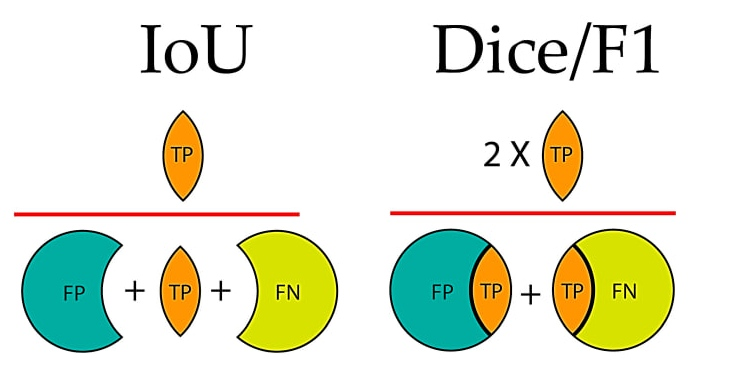
\includegraphics[width=12cm]{figuras/metrics}}}{\Fonte{\cite{maxwell2021metrics}}}
\end{figure}
\FloatBarrier{}
